\documentclass{beamer}
\usepackage[T1]{fontenc}
\usepackage[utf8]{inputenc}
\usepackage{lmodern} 
\usepackage[portuguese]{babel}
\usepackage{graphicx}			%para imagens
\usepackage{epstopdf} 			%resolve problemas eps-pdf
\usepackage{fancyhdr}			% para o cabeçalho bonito
\usepackage{caption}				%para legendas
\usepackage{placeins} 			%controlar o lugar dos floats
\usepackage{hyperref}

\defbeamertemplate*{title page}{customized}[1][]
{
  \usebeamerfont{title}\inserttitle\par
  \usebeamerfont{subtitle}\usebeamercolor[fg]{subtitle}\insertsubtitle\par
  \bigskip
 %% \usebeamerfont{author}\insertauthor\par
  \usebeamerfont{institute}\insertinstitute\par
  \usebeamerfont{date}\insertdate\par
  \usebeamercolor[fg]{titlegraphic}\inserttitlegraphic
}

%DEFINE TEMA BEAMER A SER UTILIZADO
\usetheme{Warsaw}
%DEFINIÇÃO DE TÍTULO, AUTORES .....
\title[Introdução a Computação Sônica]{ ICS - Trabalho I \\ MIDI Player}
%\title[pequeno título que vai no bottom da página]{título grande}%
\author{Juarez A.S.F. 11/0032829}
\institute{Universidade de Brasília}
\date{\today}

\begin{document}


\begin{frame}
        \titlepage
\end{frame}

\AtBeginSection[]
{
%%página com layout da sessão ao início de cada sessão
 \begin{frame}<beamer>
   \tableofcontents[currentsection,currentsubsection]
 \end{frame}
}

\begin{frame}{Requisitos}
	\frametitle{Requisitos}
    \begin{itemize}
	\item Desenvolver uma interface gráfica em Java que implemente um tocador MIDI com as funcionalidades básicas:
	\begin{itemize}
	 \item Controle Play/Pause
	 \item Stop
	 \item Posicionamento do instante inicial
	 \item Controle de volume
	 \item Exibição de parâmetros partitura da música que está sendo (ou está para ser) tocada: 
	    \begin{itemize}
	     \item fórmula de compasso
	     \item metro
	     \item andamento
	     \item armadura de tonalidade
	     \item indicação em tempo real[hh mm ss]
	    \end{itemize}
	\end{itemize}
    \end{itemize}
\end{frame}

\section{Classes Desenvolvidas}
\subsection{MidiPlayer}
\begin{frame}
	\frametitle{MidiPlayer}
	\begin{itemize}
		\item Encapsula as funcionalidades do tocador
		\item Utiliza mecanismo de composição e não de herança.
		\item atributos:
		\begin{itemize}
			\item File arqMidi
			\item Sequencer sequenciador;
			\item Sequence  sequencia;
			\item long tickPosition;
		\end{itemize}
		\item métodos de controle: play, \textbf{pause}, stop, goTo.
		\item métodos informativos: getDuracao, getResolucao ....
	\end{itemize}
\end{frame}

\subsection{LogWindow}
\begin{frame}
	\frametitle{LogWindow}
	\begin{itemize}
		\item Estende a classe JScrollPane
		\item é simplesmente uma tela de texto para reportar mensagens 
		durante o programa. Mensagens de erro são impressas em vermelho,
		de warning em amarelo....
		\item atributos:
		\begin{itemize}
			\item JTextPane logArea
		\end{itemize}
		\item métodos:
		\begin{itemize}
			\item report, reportGood, reportBad, reportWarning..
		\end{itemize}
	\end{itemize}
\end{frame}

\subsection{GUI}
\begin{frame}
	\frametitle{GUI}
	\begin{itemize}
		\item Estende a classe JFrame
		\item contém diversos componentes dos pacotes java.awt e javax.swing
		\item possui botões de play/pause e stop
		\item menu 'file' para carregar arquivo midi
		\item sliders de posicionamento para tempo e volume
		\item tabela para informar dados da partitura
	\end{itemize}
\end{frame}

\section{Interface Gráfica em JAVA}

\subsection{Componentes Utilizados}
\begin{frame}
	\frametitle{Componentes}
Alguns componentes utilizados na interface:	
	\begin{itemize}
		\item \textbf{ImageIcon, Icon e JButton} para botões
		\item \textbf{JSlider} para entrada/saída de informações de tempo
		\item \textbf{JLabel e JTable} para informações textuais
		\item \textbf{JMenu, JMenuItem e JMenuBar} para menu
		\item \textbf{JFileChooser} para navegar e carregar arquivo 
		\item \textbf{JTimer} para controlar tempo com que o JSlider é atualizado
	\end{itemize}
\end{frame}

\subsection{Layout}
\begin{frame}
  \frametitle{Composição de Layouts}
  \begin{itemize}
   \item Para posicionarmos espacialmente os componentes como desejamos, utilizamos uma composição de layouts.
   \item O layout mais externo é um BorderLayout
   \begin{figure}
	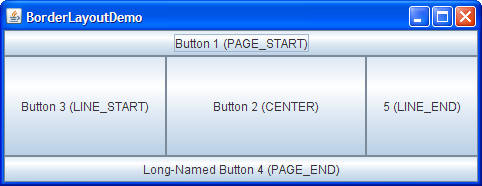
\includegraphics[scale=0.5]{./images/BorderLayout.png}
	\caption{BorderLayout}
	\label{fig:BL}
   \end{figure}
   \item Cada parte desse layout externo possui um layout próprio, como FlowLayout ou GridLayout
  \end{itemize}
\end{frame}

\begin{frame}
 \frametitle{Layouts Utilizados}
 \begin{figure}
  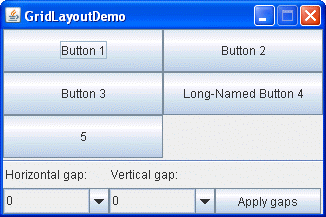
\includegraphics[scale=0.5]{./images/GridLayout.png}
  \caption{GridLayout}
 \end{figure}
 
 \begin{figure}
  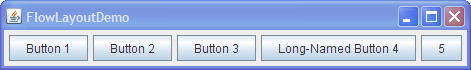
\includegraphics[scale=0.5]{./images/FlowLayout.png}
  \caption{FlowLayout}
 \end{figure} 

\end{frame}



\section{Problemas Encontrados}
\subsection{JSlider de Tempo}
\begin{frame}
    \frametitle{Slider de Tempo}
    \begin{itemize}
     \item O JSlider usado para mostrar o tempo da música possui duas funcionalidades:
     \begin{enumerate}
      \item mostrar o tempo
      \item capturar o instante em que o usuário deseja posicionar a música
     \end{enumerate}
     \item O seja, apresentas funcionalidade de entradas e saídas de dados.
     \item A alteração do seu posicionamento pode ser feita:
     \begin{enumerate}
      \item \textbf{internamente} pela controle da passagem do tempo
      \item \textbf{externamente} pelo mouse do usuário ao posicionar o slider ou ao clicar no botão stop.
     \end{enumerate}
    \item Enquanto o usuário estiver posicionando o Slider, a música continua tocando, mas deve-se desabilitar
    a passagem do tempo.
    \end{itemize}
    \end{frame}

\begin{frame}
  \frametitle{Slider de Tempo}
  \begin{itemize}
   \item Criamos uma variável controleExterno que é setada verdadeira quando o usuário está segurando
   o cursor do slider(isMoving). 
   \item Enquanto essa variável está setada, ignoramos as mudanças de relógio
   \item Quando o usuário solta o cursos, posicionamos a música no instante desejado e 
   setamos essa variável de controle para falso novamente.
  \end{itemize}
\end{frame}

\subsection{Controle Pause}
\begin{frame}
  \frametitle{Controle de Pause}
  \begin{itemize}
   \item A classe de sequenciador MIDI implementada em Java apresenta as funcionalidades:
    \begin{enumerate}
     \item start: inicia a sequência de onde estiver
     \item stop: para a sequência e seta a posição atual para seu início
     \item goto: posiciona a sequência no número de tiques desejado
    \end{enumerate}
    \item Para implementar a função de pause devemos guardar o instante atual(em tiques)
    antes de pararmos a música.
    \item Ao clicar em play novamente, devemos posicionar nesse instante salvo e então
    darmos start.
  \end{itemize}
\end{frame}






\end{document}
